\subsection{Mikrofone}
    \subsubsection{Richtcharakteristiken}
Die Richtcharakteristik gibt an, aus welcher Richtung und wie stark bzw. empfindlich ein Mikro auftreffende Schallwellen aufnimmt. Je nachdem welche Richtcharakteristik ein Mikrofon hat, ist es aus bestimmten Richtungen empfindlicher für Schall als andere Mikrofone. Mikrofone unterscheiden sich in diesem Punkt daher gar nicht so viel von dem menschlichen Gehör – auch wir haben unterschiedliche Arten zu hören und Informationen aufzunehmen: Der Schall von vorne wird lauter empfangen als der Schall von hinten (Abschattungseffekte durch Ohrmuschel).\cite{BeyerRichtchar}
\begin{center}
    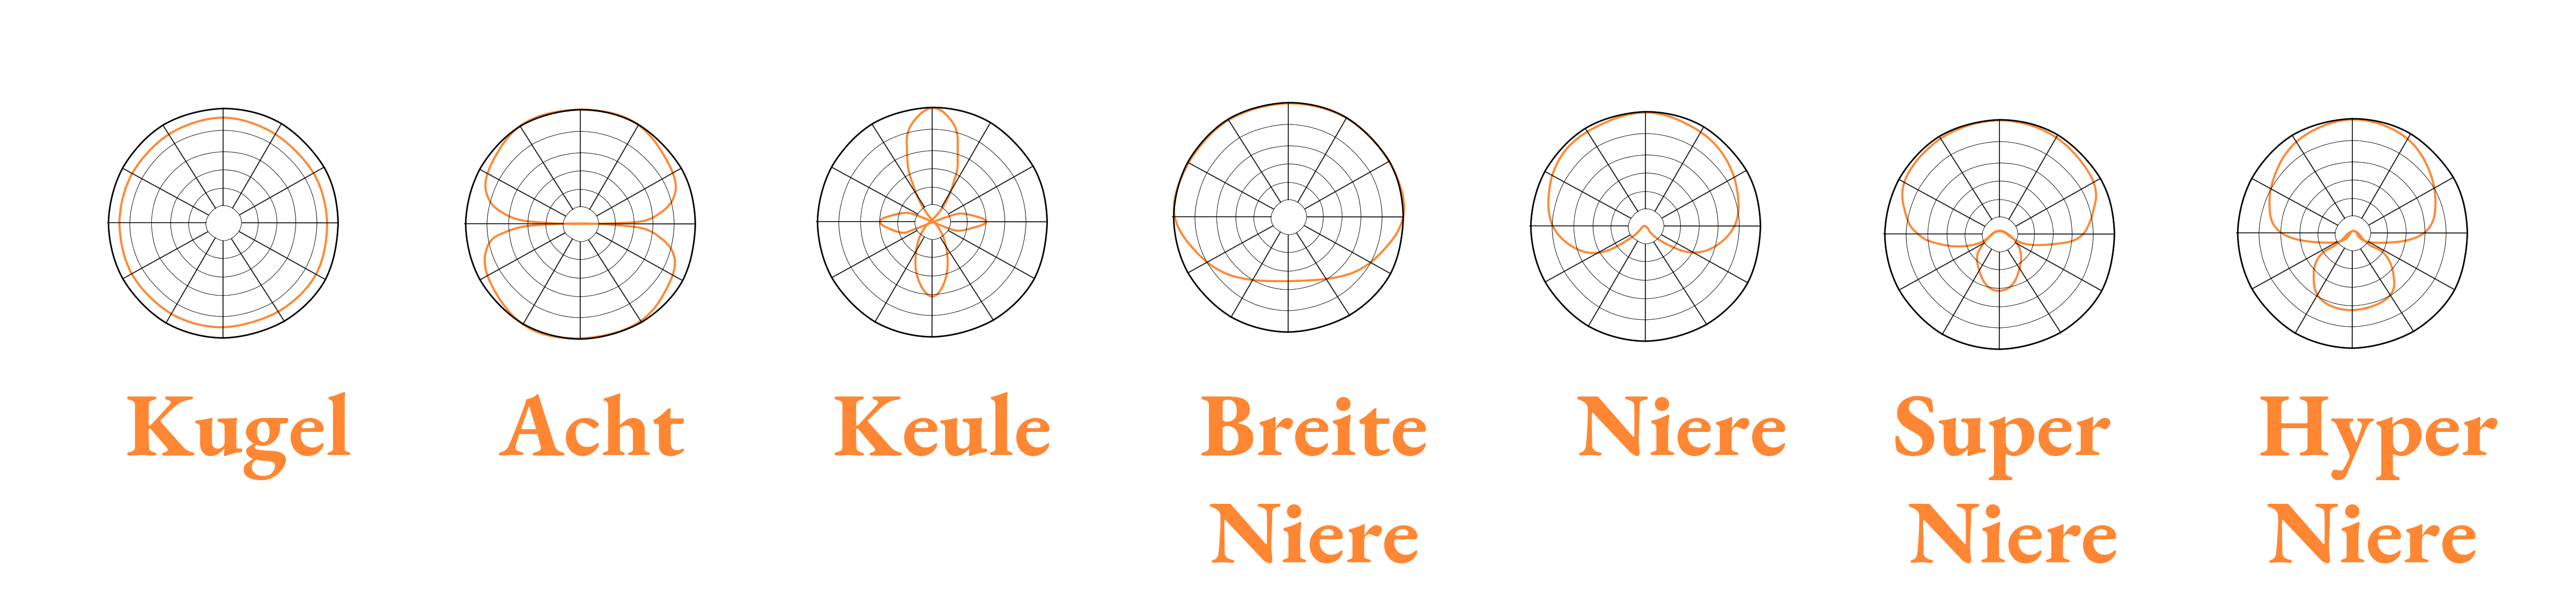
\includegraphics[width=1\textwidth]{Bilder/Medientechnik/Mikrocharakteristik.png}
\end{center}

